\documentclass[a4paper]{article}

\usepackage[utf8]{inputenc}
\usepackage[T1]{fontenc}
\usepackage{lmodern}
\usepackage[nswissgerman]{babel}
\usepackage{hyperref}
\usepackage{graphicx}
\usepackage[top=1.5cm, bottom=1.5cm, right=1.5cm, left=1.5cm]{geometry}

\title{Betriebsanleitung}
\author{Michael Schwarz}

\begin{document}

\maketitle

\section{Start-Up}
\begin{enumerate}
\item Den Verbraucher in die Buchse des Messgeräts einstecken und das Messgerät in eine Stromsteckdose einstecken.
\item Mit dem schwarzen schwarzen Schalter in Abbildung \ref{deckel} den gewünschten Strommessbereich auswählen: \\
	\begin{tabular}{c l}
		(I)  & für Ströme bis 1 A   \\
		(II) & für Ströme über 1 A. \\
	\end{tabular}
\item Leuchtet die Status-LED in Abbildung \ref{deckel} ist das Messgerät in Betrieb.
\end{enumerate}

\section{Shutdown}
\begin{enumerate}
	\item Den roten Shutdown-Taster in Abbildung \ref{deckel} links drücken, bis die LED erlischt. 
		Taster loslassen und ca. 10 s warten.
	\item Verbraucher und Messgerät trennen.
\end{enumerate}

\section{Daten auslesen}
\begin{enumerate}
	\item Computer oder Mobiltelefon mit dem W-LAN-hotspot des Messgeräts verbinden. \\
		\begin{tabular}{l l}
			SSID:     & WiPi      \\
			Passwort: & raspberry \\
		\end{tabular}
	\item Per Internetbrowser (Google Chrome oder Mozilla Firefox) auf die IP-Adresse des W-Lan-hotspots navigieren: \\
		\url{192.168.42.1}
	\item Es sollte nun die Website in Abbildung \ref{website} zu sehen sein.
	\item Für die neusten Daten muss der Browser einen hard-refresh machen: Ctrl+f5
	\item Die laufende Messung wird oben mit zwei Plots beschrieben. 
		Ältere Messdaten sind unter den Plots verlinkt.
		Die äleteren Messdaten sind als Textdateien sowie Plots verfügbar.
\end{enumerate}

\begin{figure}[h]
	\centering
	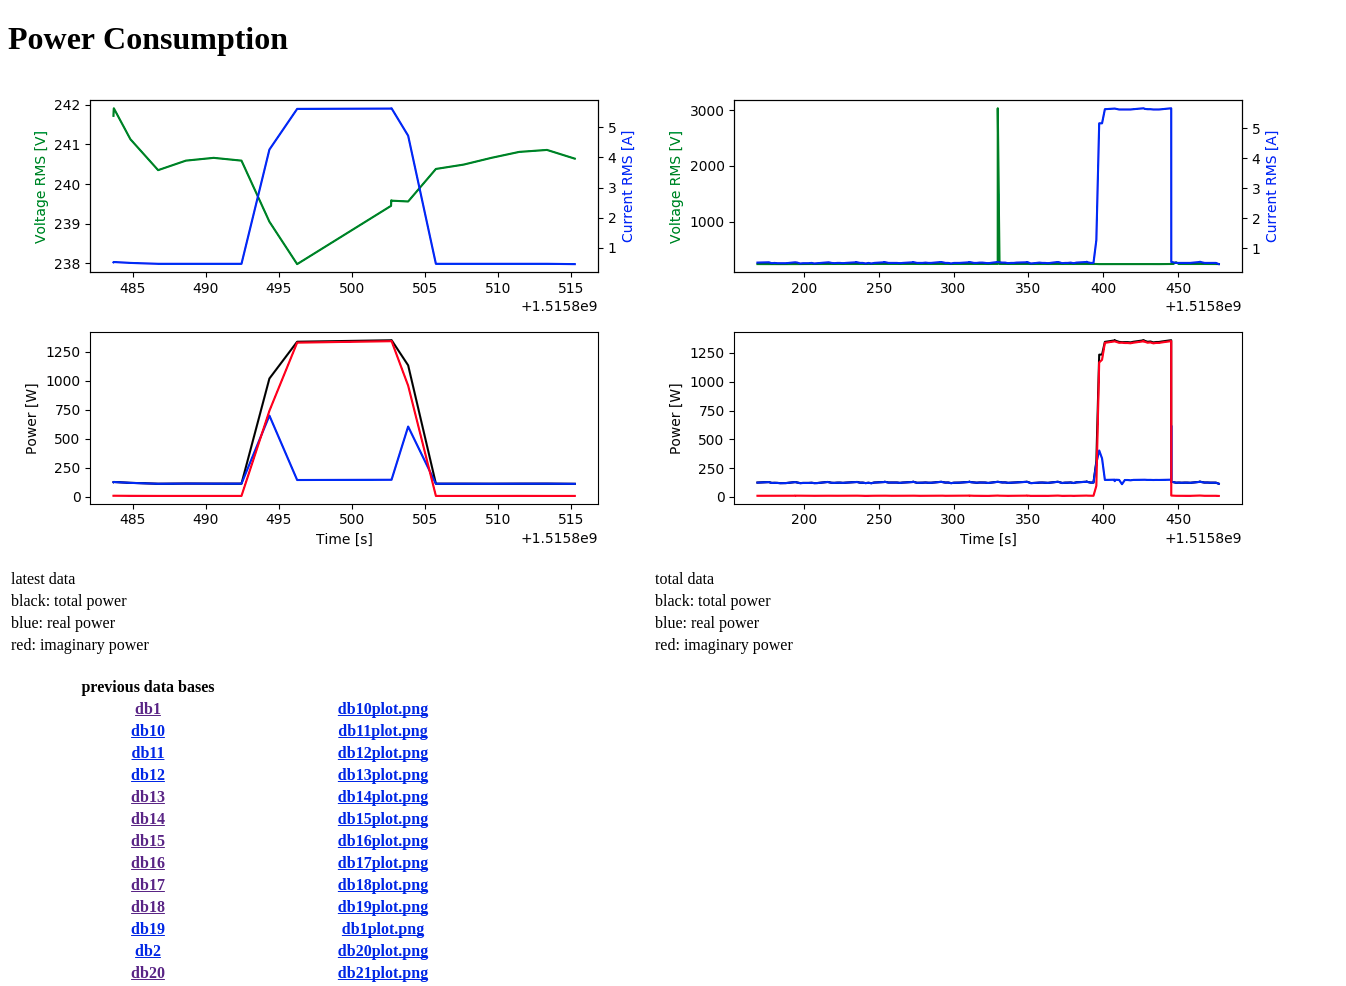
\includegraphics[width=\textwidth]{webpage_screen_dump.png}
	\caption{Website mit Daten}
	\label{website}
\end{figure}

\begin{figure}[h]
	\centering
	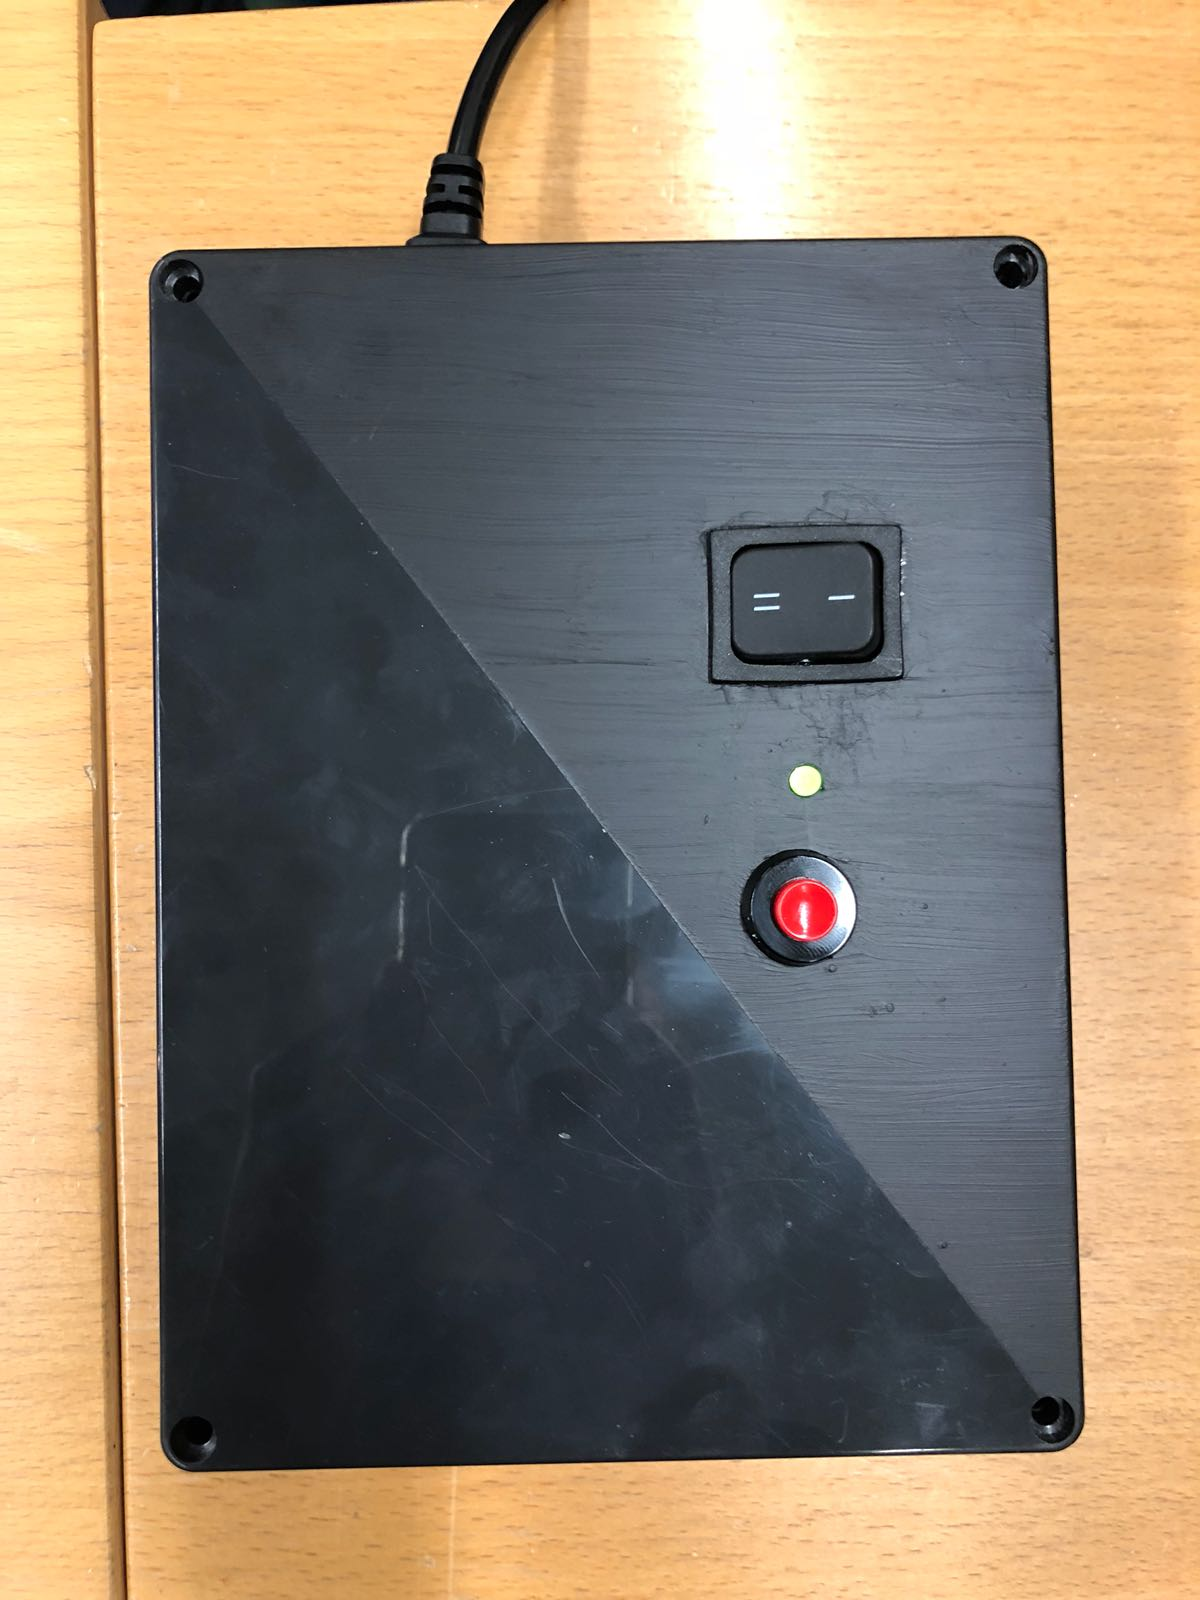
\includegraphics[width=0.5\textwidth, angle=-90]{manual_deckel.jpeg}
	\caption{Deckel des Messgeräts}
	\label{deckel}
\end{figure}

\end{document}
